\section{User Interface}

\subsection{Web-Based Front-end}

The web-based front-end of OpenPRA is designed to address the existing gaps in the current ecosystem of \acrshort{pra} tools. The front-end tries to meet a comprehensive set of requirements demanded by evolving technological landscape, including:

\begin{itemize}
\item \textbf{User friendly interface:} Provides an intuitive, browser-based \acrshort{ui} with built-in visualization tools, lowering the barrier for users of all technical backgrounds.
\item \textbf{Web based access:} Allows secure access via \acrshort{https} without client installation, supporting remote workflows.
\item \textbf{Open source platform:} Freely available and community-driven, promoting transparency, collaboration, and continuous improvement.
\item \textbf{Collaborative environment:} Enables multiple users to work concurrently on the same \acrshort{pra} model, improving teamwork and efficiency across multiple teams.
\item \textbf{Version control:} Records changes to a model, persists revision history, and supports version rollback whenever a prior state must be restored.  
\item \textbf{Support for a wide range of risk models:} Provides editors for event trees, fault trees, Markov chains, Bayesian networks, and other formalisms, enabling analysts to choose a risk model that best represents their system.  
\item \textbf{Choice of quantification engines:} Integrates multiple built-in and third-party solvers so analysts can select an algorithm most suitable for their use case.  
\item \textbf{Interoperability:} Serializes models to the standardized OpenPRA \acrshort{mef} \acrshort{json} format, ensuring seamless data exchange with external tools and workflows.
\item \textbf{Customizability:} Allows users to tailor the interface, workflows, and analysis parameters to their specific project requirements.
\end{itemize}

\begin{figure}[h!]
  \centering
  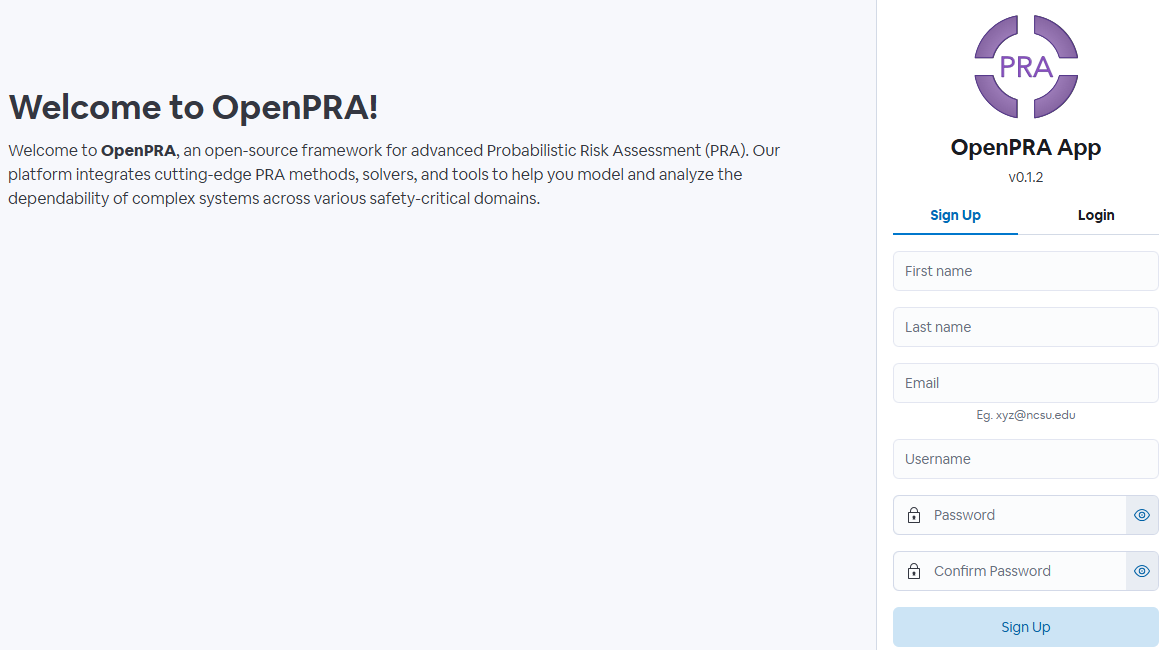
\includegraphics[width=0.9\textwidth]{4_proposed_solution/web_app/figures/landing_page.png}
  \caption{Landing page of the OpenPRA web application.}
  \label{fig:landing_page}
\end{figure}

\subsection{Analysis Modes, Types and Risk Models}

The front-end supports a wide range of analysis modes, analysis types and risk models. This enables users to tailor their risk assessment process to their specific needs and preferences. An overview of the supported analysis modes have been given below. Figures \ref{fig:analysis_modes_types}, \ref{fig:data_analysis}, and \ref{fig:analysis_modes} show overviews of internal event and data analyses, and different analysis modes supported by the v2 app.

\begin{itemize}
  \item \textbf{Internal events analysis:} Helps to model events originating within the system such as equipment failures or operator errors, to assess their impact on overall reliability and safety of the system.
  \item \textbf{Internal hazards analysis:} Provides tools to model hazards arising inside the system e.g., fires or floods, and evaluates their potential risk to system integrity.
  \item \textbf{External hazards analysis:} Supports the modeling of external events such as earthquakes, to determine their effects on system performance and safety.
  \item \textbf{Full scope \acrshort{pra} analysis:} Offers a comprehensive analysis of all potential risks, integrating modeling of both internal and external events and hazards.
  \item \textbf{Data analysis:} Enables importing, processing, and analyzing system data such as failure and operational records, using parametric distributions (e.g., from \acrshort{nrc} industry average parameter estimates database) to gain insights into system performance and reliability.
\end{itemize}

Aside from data analysis, each of the listed analysis modes supports the analysis types:

\begin{itemize}
  \item \textbf{Plant operating states analysis:} Analyzes system performance and reliability across different plant modes such as full power, low power, and shutdown to identify plant-state specific risk profiles.
  \item \textbf{Initiating events analysis:} Models and assesses internal or external triggers like equipment failures, human errors, and natural disasters to evaluate their potential to initiate accident sequences.
  \item \textbf{Event sequence analysis:} Analyzes the chain of events following an initiating event to evaluate possible failure pathways and their associated probabilities.
  \item \textbf{Success criteria development:} Defines metrics for successful system operation and assesses the likelihood of meeting these criteria under various operating conditions and event scenarios.
  \item \textbf{System analysis:} Uses modeling techniques such as fault tree analysis and reliability block diagrams to evaluate overall system performance under failure and hazard conditions.
  \item \textbf{Human reliability analysis:} Assesses the impact of active and latent human errors on system safety using an \acrshort{hra} methodology extended from Phoenix.
  \item \textbf{Mechanistic source term analysis:} Models and assesses the release mechanisms of hazardous materials during an accident to determine source terms.
  \item \textbf{Radiological consequence analysis:} Models dispersion and assesses exposure of radioactive materials post-accident to quantify potential radiological impacts on workers and the public.
  \item \textbf{Uncertainty analysis:} Applies parametric, non-parametric, and Monte Carlo sampling methods to assess uncertainties in risk assessment inputs and outputs.
  \item \textbf{Risk integration analysis:} Integrates results from individual analyses and models overall system risk as frequency-consequence curves for a comprehensive risk profile.
\end{itemize}

\begin{figure}
  \centering
  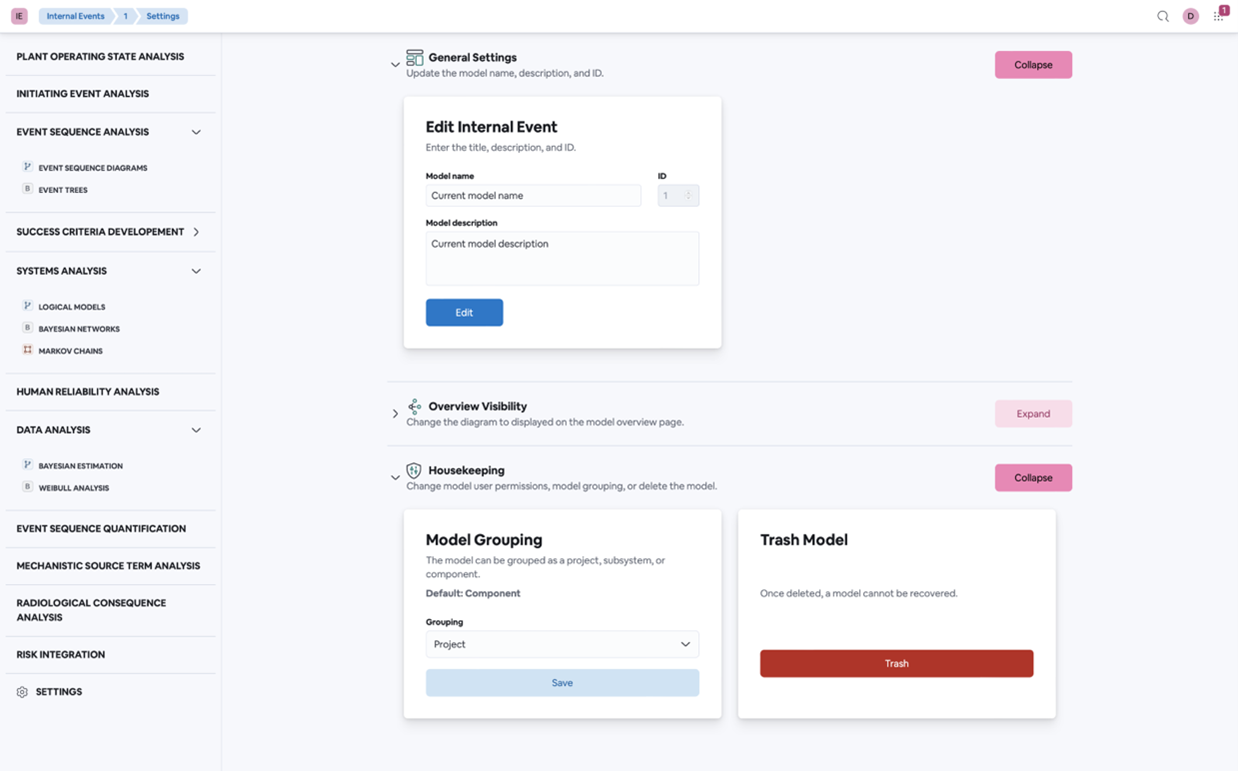
\includegraphics[width=1.0\textwidth]{4_proposed_solution/web_app/figures/analysis_modes_types.png}
  \caption{Internal events analysis overview.}
  \label{fig:analysis_modes_types}
\end{figure}

\begin{figure}
  \centering
  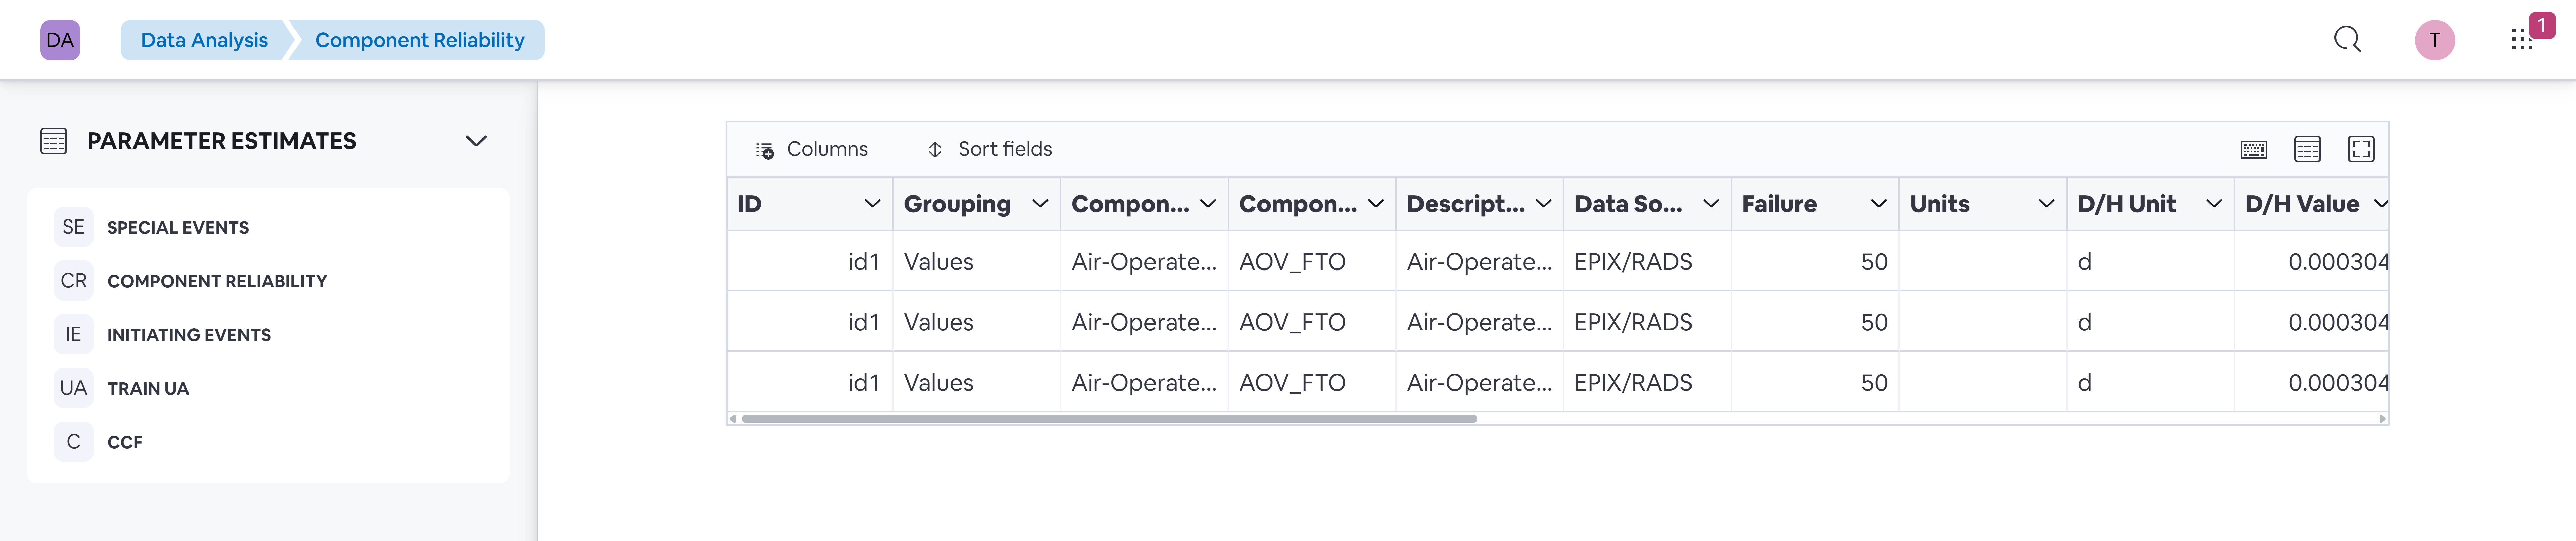
\includegraphics[width=1.0\textwidth]{4_proposed_solution/web_app/figures/data_analysis.png}
  \caption{Data analysis overview.}
  \label{fig:data_analysis}
\end{figure}

\begin{figure}
  \centering
  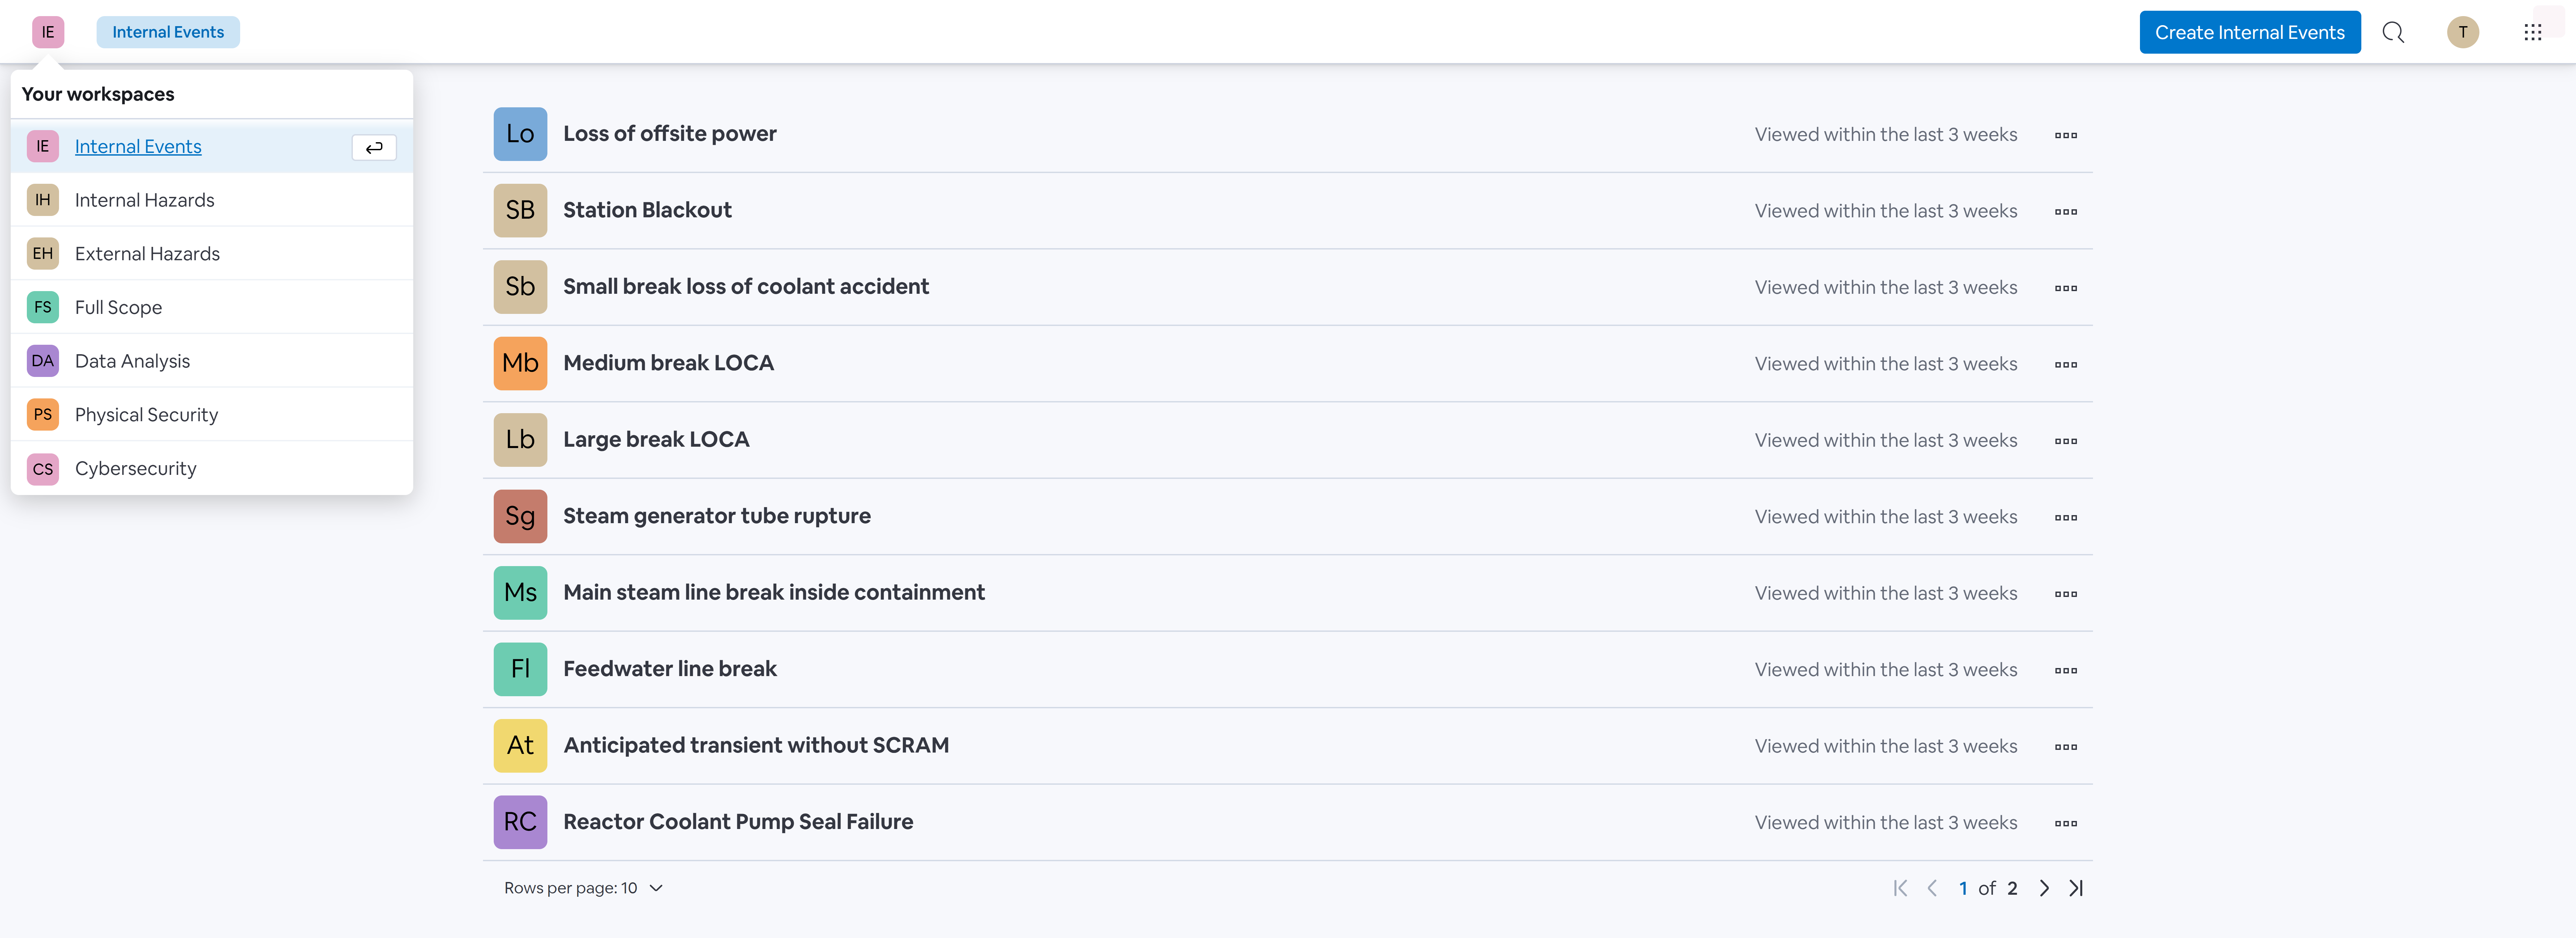
\includegraphics[width=1.0\textwidth]{4_proposed_solution/web_app/figures/analysis_modes.png}
  \caption{Analysis modes supported by the v2 app.}
  \label{fig:analysis_modes}
\end{figure}

The front-end supports a wide array of risk models, each designed to address specific components of the analysis types outlined earlier. Figures \ref{fig:pos_editor} through \ref{fig:bn_editor} show such six risk models.

\begin{itemize}
  \item \textbf{Initiating events:} Models and assesses potential triggers using master logic diagrams, \acrshort{fmea}, and heat balance fault trees for internal or external failures (e.g., equipment failures, human errors, natural disasters) that can shift the system into accident sequences.
  \item \textbf{Event sequence diagrams:} Provides compressed-notation diagrams with support for cycles to model and analyze complex, temporally arranged phenomena following an initiating event.
  \item \textbf{Event trees:} Uses node and branch based diagrams to model and analyze possible sequences of events leading to specific outcomes, assessing the likelihood and consequences of each pathway.
  \item \textbf{Fault trees:} Employs Boolean gate and basic event based diagrams to model combinations of component failures and analyze their contributions to overall system failure.
  \item \textbf{Markov chains:} Applies probabilistic state transition models to analyze system reliability and availability over time through discrete states and transitions.
  \item \textbf{Bayesian networks:} Constructs directed graph models of probabilistic dependencies to analyze uncertain variables and their interactions within complex systems.
  \item \textbf{Probabilistic model checkers:} Integrates dual-graph error propagation models to model and analyze the propagation of faults, errors, and failures through a cyber-physical system.
  \item \textbf{Consequence models:} Links end states of event sequences with categorized outcomes (e.g., radiological doses, financial losses) and integrates them into frequency-consequence curves for comprehensive risk evaluation.
\end{itemize}

%--------------------------------------------------------------
\begin{figure}
  \centering
  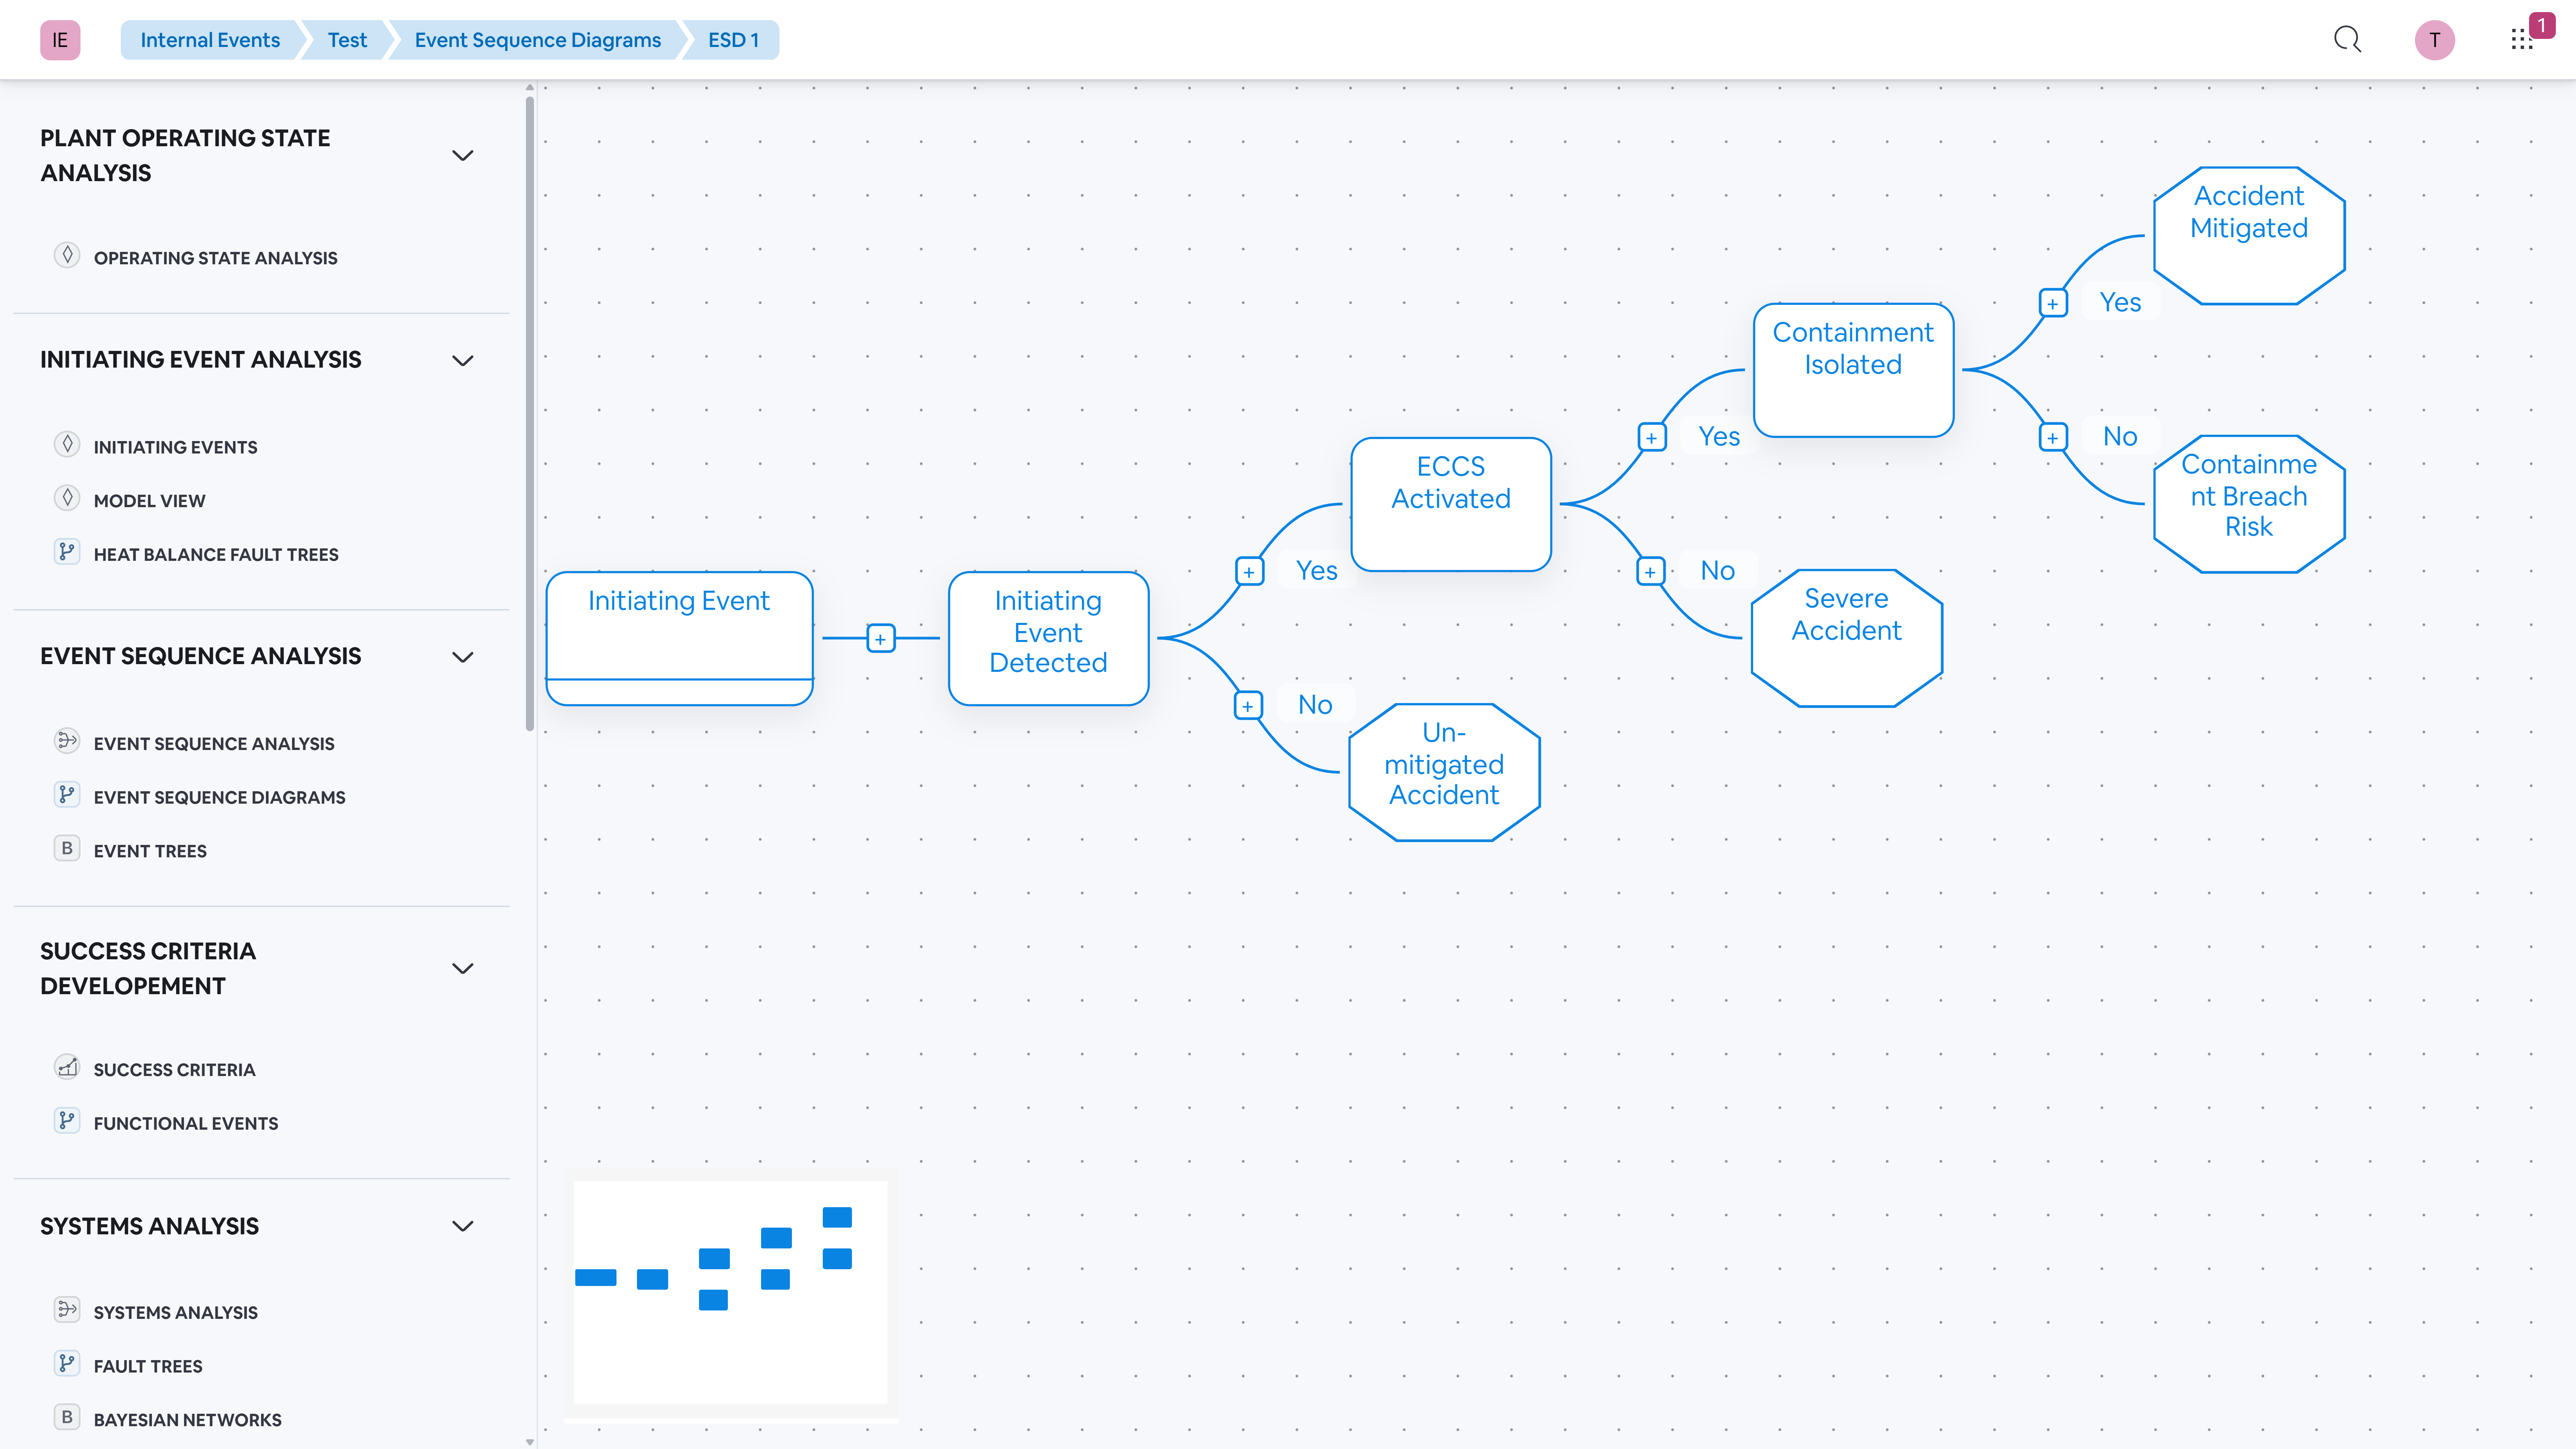
\includegraphics[width=\textwidth]{4_proposed_solution/web_app/figures/esd.png}
  \caption{Event sequence diagram editor.}
  \label{fig:esd_editor}
\end{figure}

%--------------------------------------------------------------
\begin{figure}
  \centering
  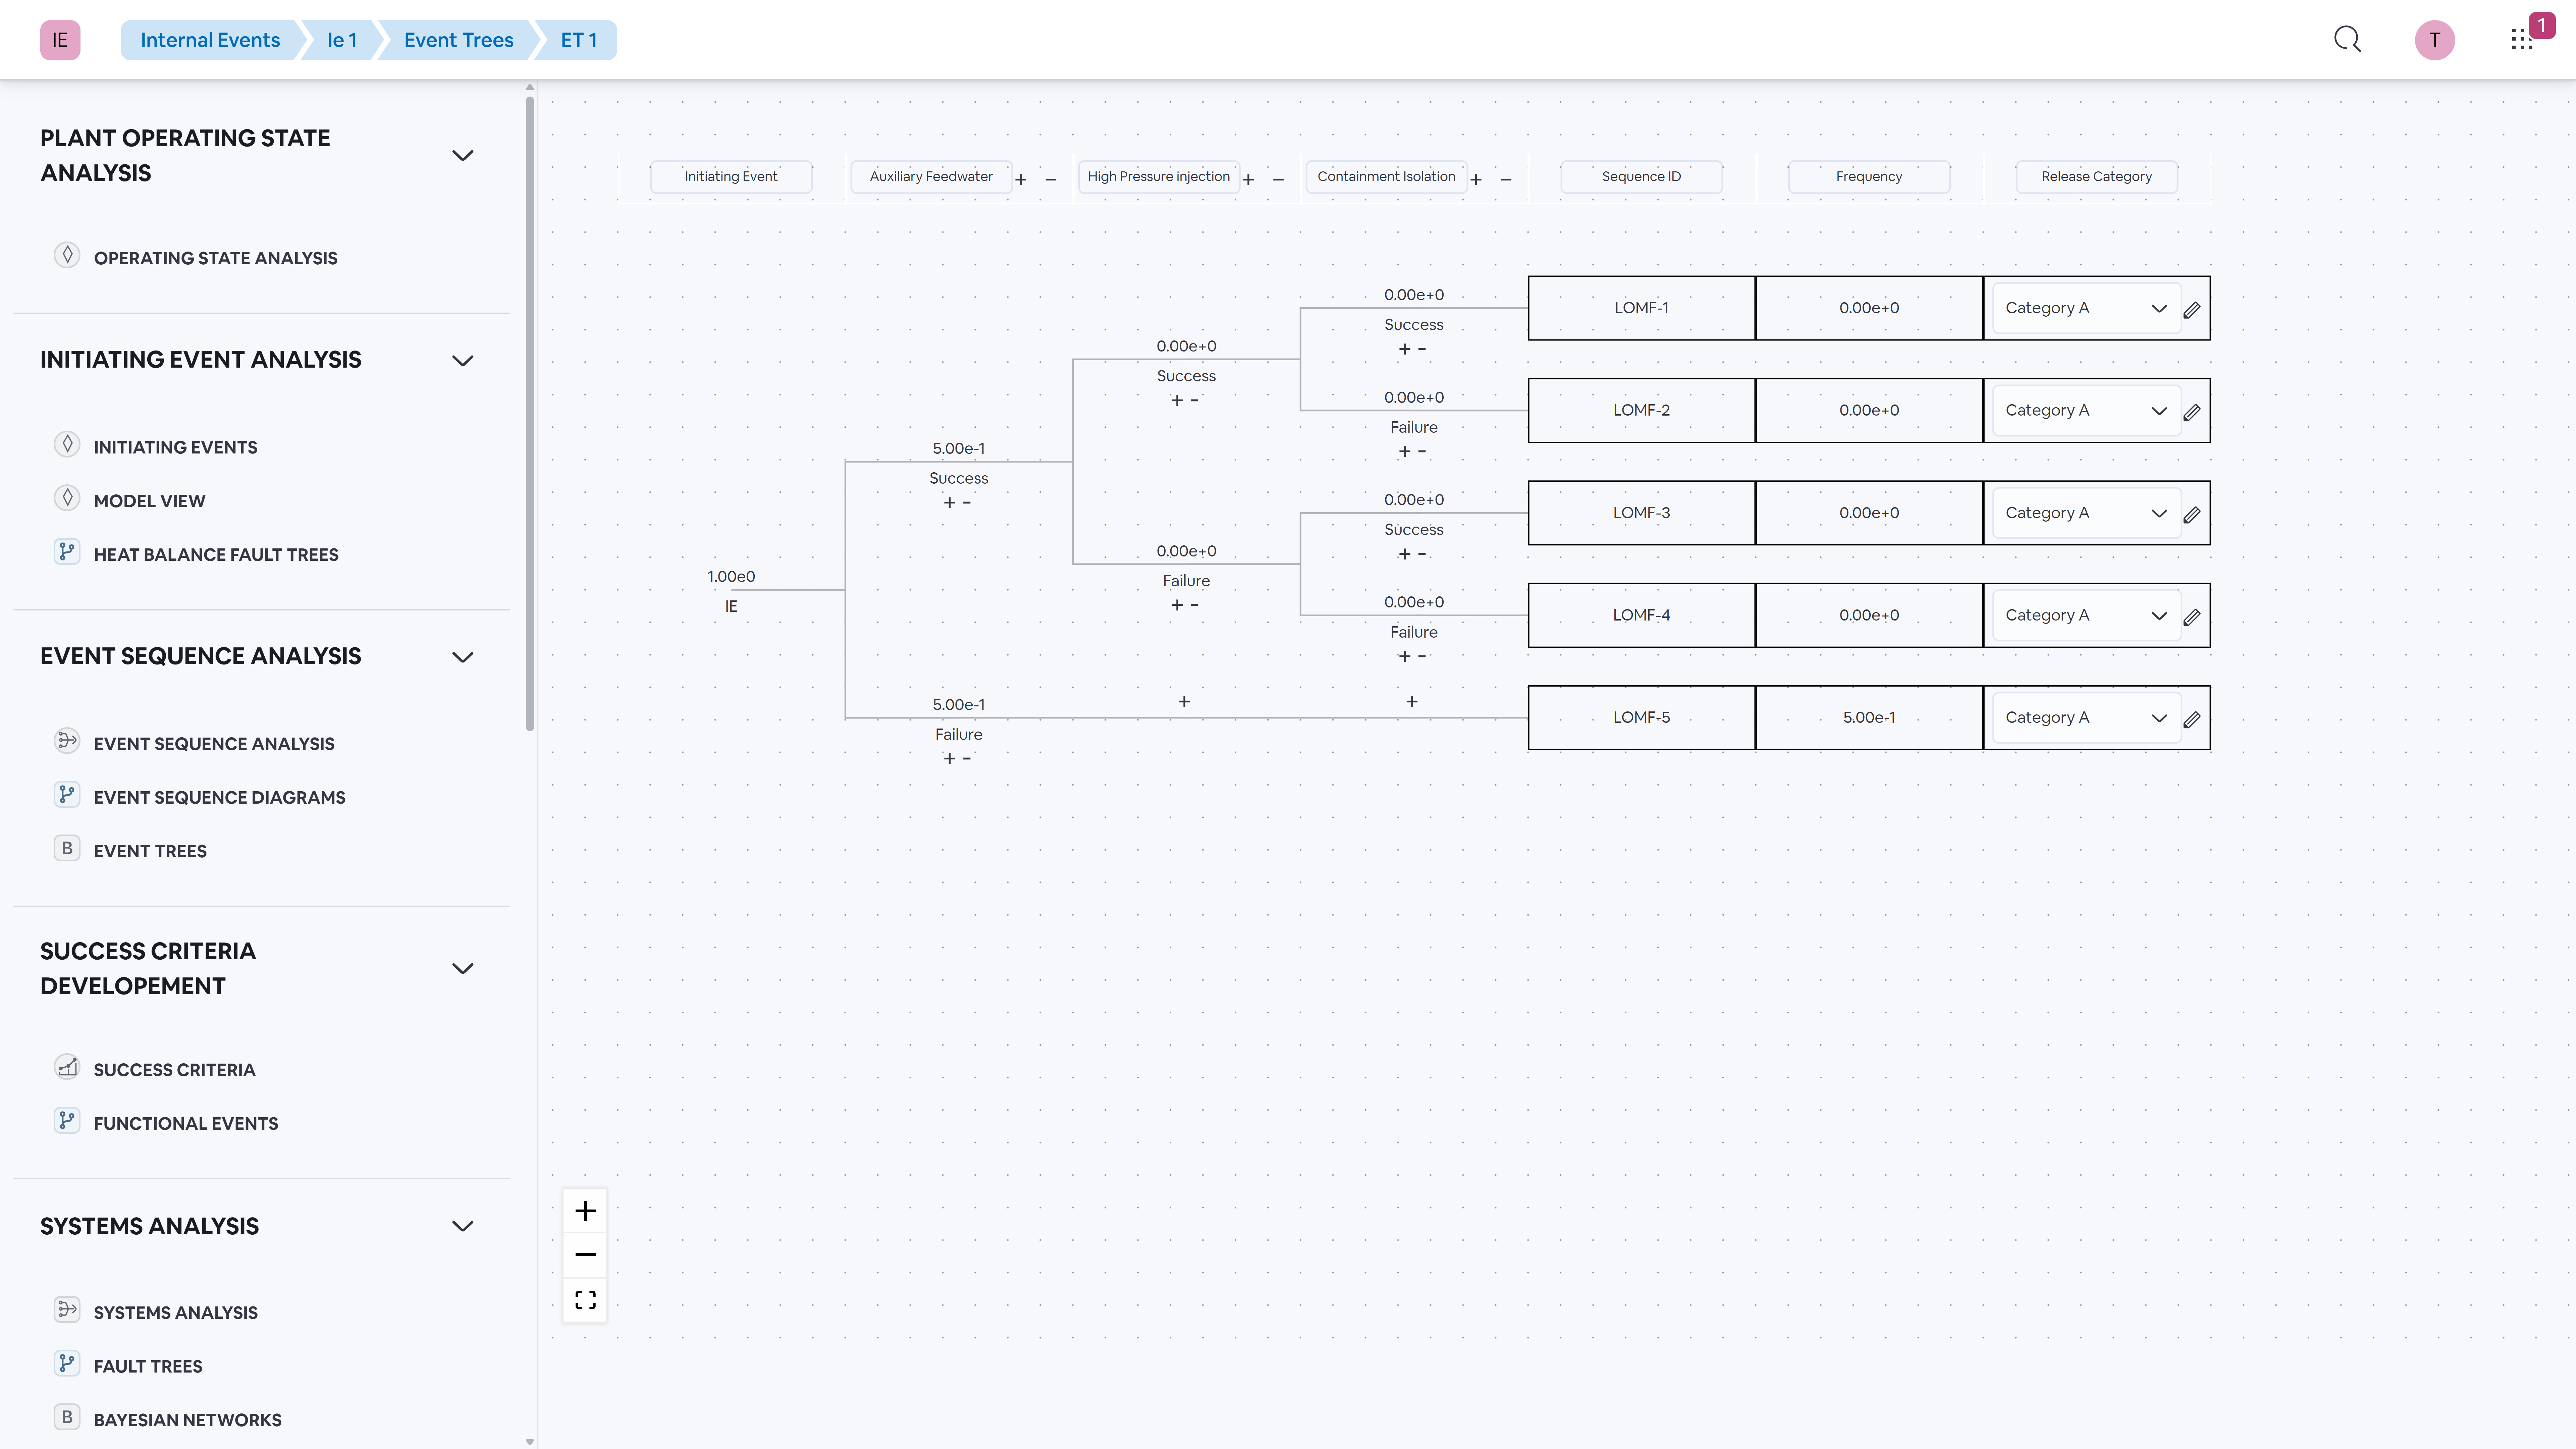
\includegraphics[width=\textwidth]{4_proposed_solution/web_app/figures/et.png}
  \caption{Event tree editor.}
  \label{fig:et_editor}
\end{figure}

%--------------------------------------------------------------
\begin{figure}
  \centering
  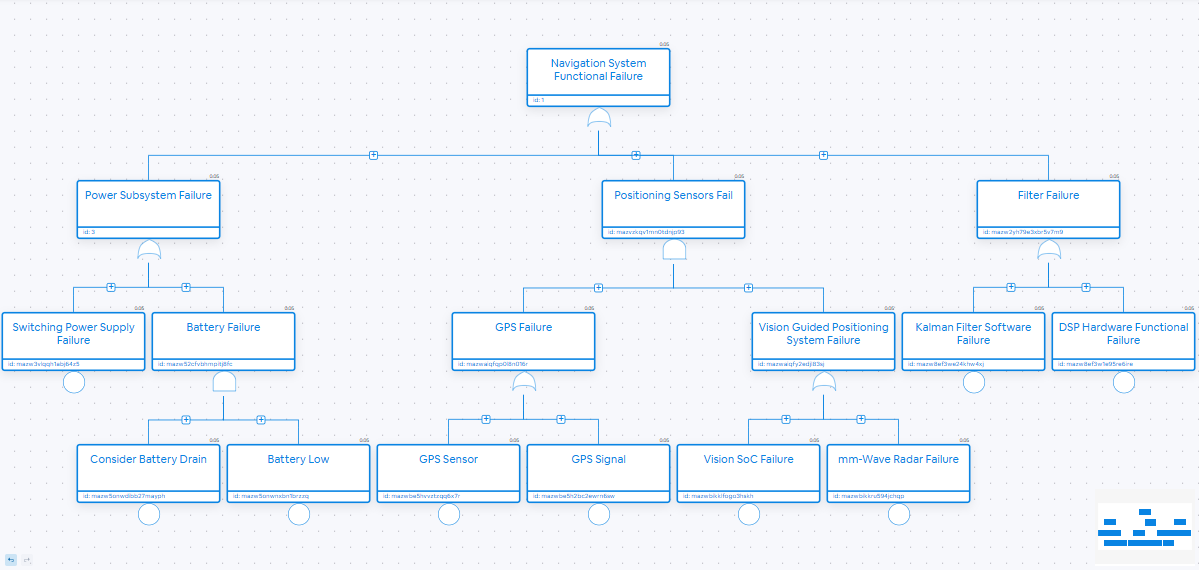
\includegraphics[width=\textwidth]{4_proposed_solution/web_app/figures/ft.png}
  \caption{Fault tree editor.}
  \label{fig:ft_editor}
\end{figure}

%--------------------------------------------------------------
\begin{figure}
  \centering
  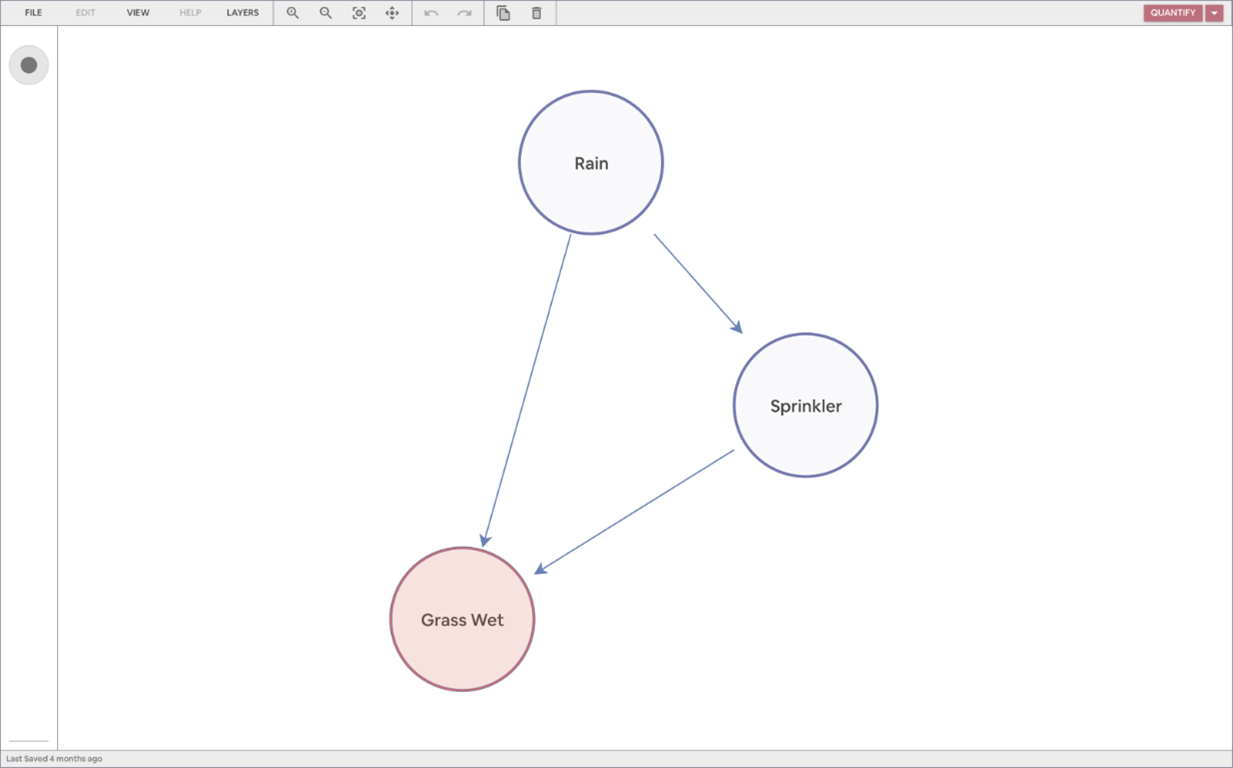
\includegraphics[width=\textwidth]{4_proposed_solution/web_app/figures/bn.png}
  \caption{Bayesian network editor.}
  \label{fig:bn_editor}
\end{figure}

OpenPRA currently uses \acrshort{hcla} as its default analyzer but is transitioning to the scram engine, with plans to phase out \acrfull{hcla} due to its proprietary license. To support advanced users, developers, and industry partners, OpenPRA offers \acrfull{api}s, tooling, and integration guides for adding custom or third-party engines enabling on-premise deployments and accommodating specific licensing requirements. Users can choose among multiple quantification engines when solving risk models. The front-end provides interfaces for the following solvers:

\begin{itemize}
  \item \textbf{scram:} A command-line tool for quantifying models specified in the OpenPSA \acrshort{mef} \acrshort{xml} schema. It implements \acrshort{bdd} for exact probability calculations, \acrshort{mocus}, along with \acrshort{mcub} and \acrshort{rea}, and \acrshort{zdd}, and supports uncertainty analysis via Monte Carlo simulation, importance analysis, and common cause failure groups (CCFGs).
  \item \textbf{XFTA:} Provides advanced fault tree quantification algorithms including cut-set enumeration, \acrshort{mcs} generation, and importance analysis and implements \acrshort{bdd}, \acrshort{mocus}, and \acrshort{zdd} in version 2 and above.
  \item \textbf{Saphsolve:} The proprietary engine behind \acrshort{saphire}, supporting event tree analysis, fault tree analysis, and uncertainty analysis through its suite of quantification algorithms.
  \item \textbf{PRAQuant:} The default, proprietary fault tree quantification engine in Phoenix Architect, optimized for detailed fault tree analysis.
  \item \textbf{FTREX:} An optional, proprietary Phoenix Architect engine for fault tree quantification that offers additional algorithm choices.
  \item \textbf{Custom quantification engines:} Enables users to develop and integrate custom engines written in C++, Python, Java, etc. via OpenPRA's \acrfull{api}s, allowing tailored quantification workflows.
\end{itemize}

\begin{figure}[h!]
  \centering
  \begin{subfigure}[b]{0.49\textwidth}
    \centering
    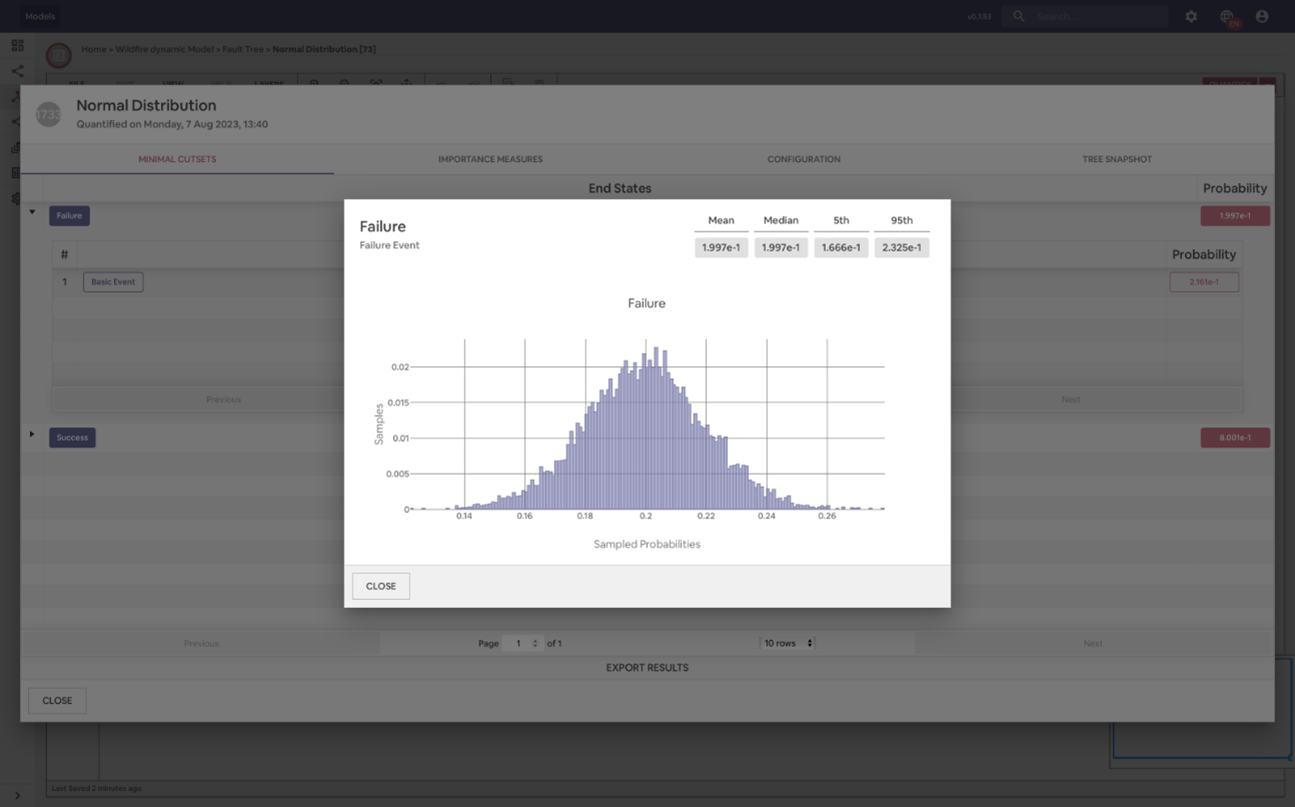
\includegraphics[width=\textwidth]{4_proposed_solution/web_app/figures/cutsets_uncertainty.png}
    \caption{}
  \end{subfigure}
  \begin{subfigure}[b]{0.49\textwidth}
    \centering
    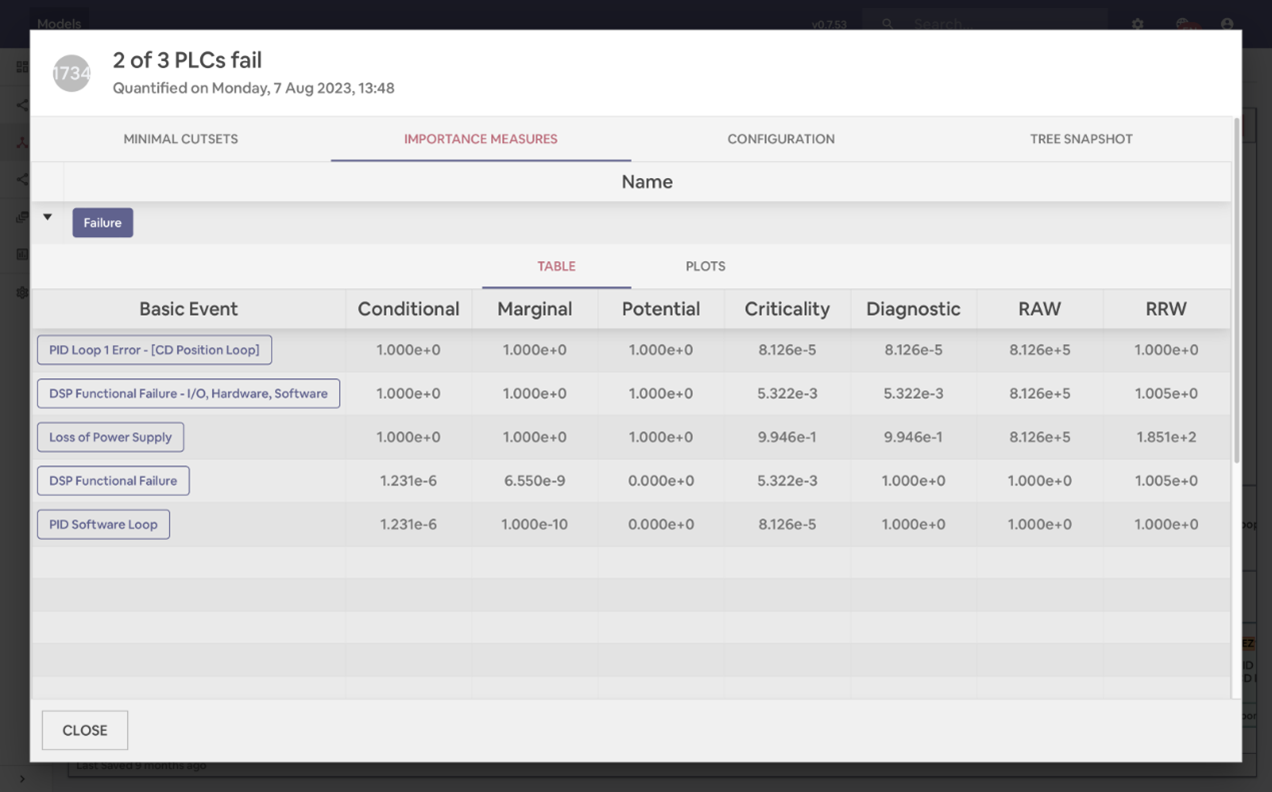
\includegraphics[width=\textwidth]{4_proposed_solution/web_app/figures/importance.png}
    \caption{}
  \end{subfigure}
  \begin{subfigure}[b]{0.49\textwidth}
    \centering
    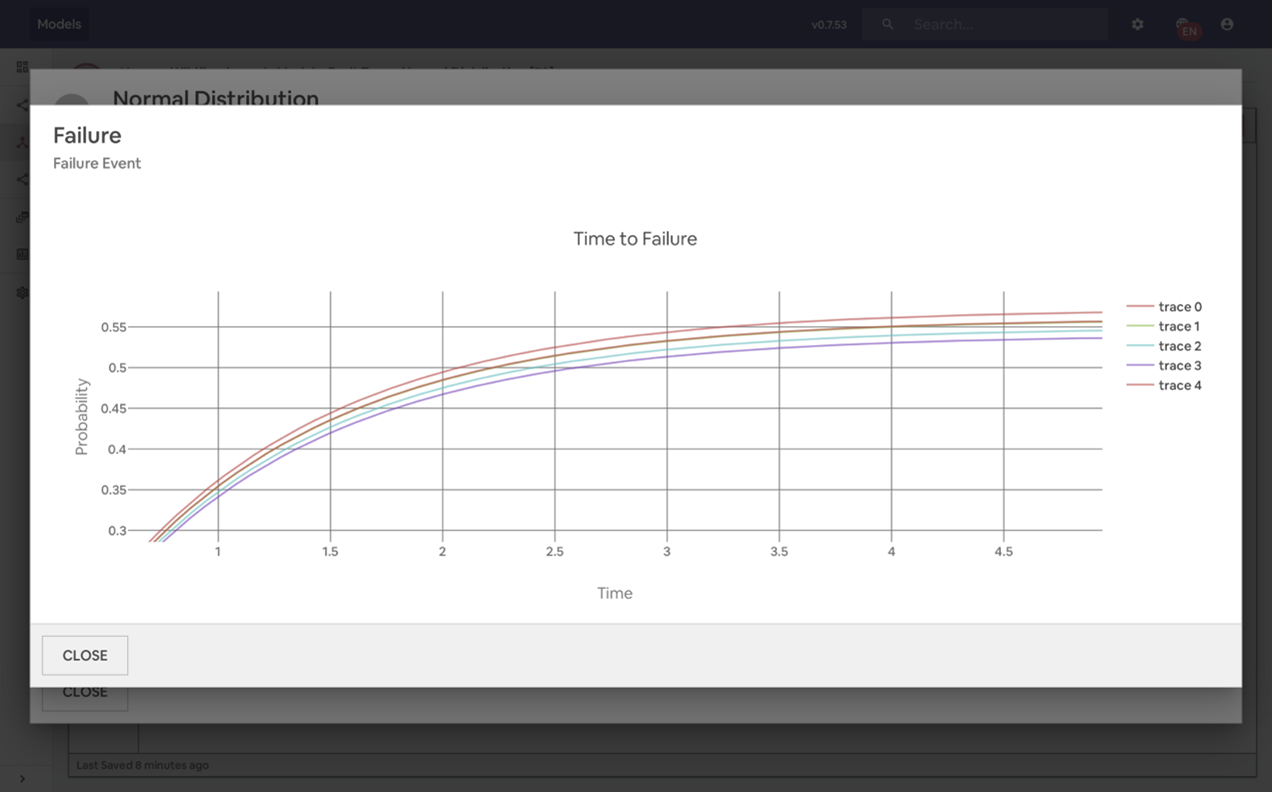
\includegraphics[width=\textwidth]{4_proposed_solution/web_app/figures/ttf.png}
    \caption{}
  \end{subfigure}
  \caption{(a) Cut sets, uncertainty using Monte Carlo sampling, (b) Importance measures calculation, (c) Time to failure cumulative distribution function with uncertainty quantification.}
  \label{fig:quantification_results}
\end{figure}